% !TEX root = doc.tex
% Copyright (c) 2017 The ALF project.
% This is a part of the ALF project documentation.
% The ALF project documentation by the ALF contributors is licensed
% under a Creative Commons Attribution-ShareAlike 4.0 International License.
% For the licensing details of the documentation see license.CCBYSA.
%
%-----------------------------------------------------------------------------------
\subsection{Stabilization - a peculiarity of the BSS algorithm}\label{sec:stable}
%-----------------------------------------------------------------------------------
%
From the partition function in Eq.~\eqref{eqn:partition_2} it can be seen that, for the calculation of the Monte Carlo weight and of the observables, a long product of matrix exponentials has to be formed.
In addition to that, we need to be able to extract the single-particle Green function  for a given flavor index at, say, time slice $\tau = 0$.  As  mentioned above (cf. Eq.~\eqref{eqn:Green_eq}), this quantity is given by: 
\begin{equation}
\bm{G}= \left( \mathds{1} + \prod_{ \tau= 1}^{L_{\text{Trotter}}} \bm{B}_\tau \right)^{-1},
\end{equation}
which can be recast as the more familiar linear algebra problem of finding a solution for the linear system
\begin{equation}
\left(\mathds{1} + \prod_\tau \bm{B}_\tau\right) x = b.
\end{equation}
The matrices $\bm{B}_\tau \in \mathbb{C}^{n\times n}$ depend on the lattice size as well as other physical parameters that can be chosen such that a matrix norm of $\bm{B}_\tau$ can be unbound in size.
From standard perturbation theory for linear systems, the computed solution $\tilde{x}$ would 
contain a relative error
\begin{equation}
\frac{|\tilde{x} - x|}{|x|} = \mathcal{O}\left(\epsilon \kappa_p\left(\mathds{1} + \prod_\tau \bm{B}_\tau\right)\right),
\end{equation}
where $\epsilon$ denotes the machine precision, which is $2^{-53}$ for IEEE double-precision numbers, and $\kappa_p(\bm{M})$ is the condition number of the matrix $\bm{M}$ with respect to the matrix $p$-norm. Due to $\prod_ \tau \bm{B}_\tau$ containing exponentially large and small scales, as can be seen in Eq.~\eqref{eqn:partition_2}, a straightforward inversion turns out to be completely ill-suited. That would lead the condition number, as a function of increasing inverse temperature, to grow exponentially, rendering the computed solution $\tilde{x}$ meaningless.

In order to circumvent this, more sophisticated methods have to be employed. As a first step, assuming that the multiplication of \texttt{NWrap} $\bm{B}$ matrices has an acceptable condition number and, for simplicity, that \texttt{NWrap} is a divisor of $L_{\text{Trotter}}$, we can write:
%\begin{equation}
%\bm{G} = \left( \mathds{1} + \prod\limits_{ i = 0}^{\frac{L_{\text{Trotter}}} {\texttt{NWrap} -1}}       \underbrace{\prod_{\tau=1}^{\texttt{NWrap}} \bm{B}_{i  \cdot  \texttt{NWrap}+ \tau} }_{ \equiv \mathcal{\bm{B}}_i}\right)^{-1}.
%\end{equation}
\begin{equation}
\bm{G} = \left( \mathds{1} + \prod\limits_{ i = 1}^{\frac{L_{\text{Trotter}}} {\texttt{NWrap}}}       \underbrace{\prod_{\tau=1}^{\texttt{NWrap}} \bm{B}_{(i-1)  \cdot  \texttt{NWrap}+ \tau} }_{ \equiv \mathcal{\bm{B}}_i}\right)^{-1}.
\end{equation}
The default stabilization strategy in the auxiliary-field QMC implementation of the ALF project, is then to form a product of QR-decompositions, which was proven to be weakly backwards stable in \cite{Bai2011}.
The key idea is to efficiently separate the scales of a matrix from the orthogonal part of a matrix.
This can be achieved using a QR decomposition of a matrix $\bm{A}$ in the form $\bm{A}_i = \bm{Q}_i \bm{R}_i$. The matrix $\bm{Q}_i$ is unitary and hence in the usual $2$-norm it holds that $\kappa_2(\bm{Q}_i) = 1$.
To get a handle on the condition number of $\bm{R}_i$ we will form the
diagonal matrix
\begin{equation}
(\bm{D}_i)_{n,n} = |(\bm{R}_i)_{n,n}|
\label{eq:diagnorm}
\end{equation}
and set $\tilde{\bm{R}}_i = \bm{D}_i^{-1} \bm{R}_i$
This gives the decomposition
\begin{equation}
\bm{A}_i = \bm{Q}_i \bm{D}_i \tilde{\bm{R}}_i.
\end{equation}
$\bm{D}_i$ now contains the row norms of the original $\bm{R}_i$ matrix and hence attempts to separate off the total scales of the problem from $\bm{R}_i$.
This is similar in spirit to the so-called matrix equilibration which tries to improve the condition number of a matrix through suitably chosen column and row scalings.
Due to a theorem by van der Sluis \cite{vanderSluis1969} we know that the choice in Eq.~\eqref{eq:diagnorm} is almost optimal among all diagonal matrices $\bm{D}$ from the space of diagonal matrices $\mathcal{D}$, in the sense that
\begin{equation*}
\kappa_p((\bm{D}_i)^{-1} \bm{R}_i ) \leq n^{1/p} \min_{\bm{D} \in \mathcal{D}} \kappa_p(\bm{D}^{-1} \bm{R}_i).
\end{equation*}
Now, given an initial decomposition of $\bm{A}_{j-1} = \prod_i \mathcal{\bm{B}}_i = \bm{Q}_{j-1} \bm{D}_{j-1} \bm{T}_{j-1}$ an update
$\mathcal{\bm{B}}_j \bm{A}_{j-1}$ is formed in the following three steps:
\begin{enumerate}
\item Form $ \bm{M}_j = (\mathcal{\bm{B}}_j \bm{Q}_{j-1}) \bm{D}_{j-1}$. Note the parentheses.
\item Do a QR decomposition of $\bm{M}_j = \bm{Q}_j \bm{D}_j \bm{R}_j$. This gives the final $\bm{Q}_j$ and $\bm{D}_j$.
\item Form the updated $\bm{T}$ matrices $\bm{T}_j = \bm{R}_j \bm{T}_{j-1}$.
\end{enumerate}
%While this provides provides a stable method to calculate the involved matrix product
%it can be pretty expensive. Therefore the user can specify to skip a certain number of 
%QR Decompositions and perform plain multiplications instead. This is specified in the parameters file by the \path{NWrap} parameter.
%\path{NWrap}~=~1 corresponds to always performing QR decompositions whereas larger integers give longer intervals where no QR decomposition will be performed.
The effectiveness of the stabilization \emph{has} to be judged for every simulation from the output file \path{info} (Sec.~\ref{sec:output_obs}). For most simulations there are two values to look out for:
\begin{itemize}
\item \texttt{Precision Green}
\item \texttt{Precision Phase}
\end{itemize}
The Green function, as well as the average phase, are usually numbers with a magnitude of $\mathcal{O} (1)$. 
For that reason we recommend that \path{NWrap} is chosen such that the mean precision is of the order of $10^{-8}$ or better (or further recommendations see Sec.~\ref{sec:optimize}).
We include typical values of \texttt{Precision Phase} and of the mean and the maximal values of \texttt{Precision Green} in the example simulations discussed in Sec.~\ref{sec:prec_charge} and Sec.~\ref{sec:prec_spin}.


%-----------------------------------------------------------------------------------
\subsection{The Trotter error and  checkerboard  decomposition }\label{sec:hermitian}
%-----------------------------------------------------------------------------------
%

In practice, many applications are carried out at finite  imaginary time steps,  and it is important to  understand the consequences of the Trotter error.   How does it scales with system size and  what  symmetries  does it  breaks?   In particular, if  one is investigating a critical  point, then one should understand  if the potential symmetry breaking  associated  with the Trotter decomposition   generates  relevant operators. 

To at best describe the workings of the ALF  code,  we divide the Hamiltonian into  hopping terms  $\hat{\mathcal{H}}_{T}$  and into interaction terms  
$\hat{\mathcal{H}}_{V} +  \hat{\mathcal{H}}_{I}   +   \hat{\mathcal{H}}_{0,I} $.       Let 
\begin{equation}
	\hat{\mathcal{H}}_{T}     = \sum_{i=1}^{N_T} \sum_{k \in \mathcal{S}^{T}_i} \hat{T}^{(k)}  \equiv \sum_{i=1}^{N_T} \hat{T}_{i} 
\end{equation}
Here the decomposition follows the rule  that if $k$ and $k'$  belong to the same set $\mathcal{S}^{T}_i $ the   $ \left[ \hat{T}^{(k)} , \hat{T}^{(k')} \right] = 0 $.  As an 
example, we can mention the checkerboard decomposition.   For the square lattice we can decouple the nearest neighbor hopping  into $N_T=4$ groups,  each group consisting  sum  of two site hopping processes.    This type of checkerboard decomposition is activated for a set  of predefined lattices provided that the flag 
\texttt{Checkerboard}   is activated.     
We will carry out the same decomposition for the interaction: 
\begin{equation}
	\hat{\mathcal{H}}_{V}  +  \hat{\mathcal{H}}_{I}   +   \hat{\mathcal{H}}_{0,I}   = \sum_{i=1}^{N_I}  \hat{O}_{i}
\end{equation}
where $\hat{O}_{i}$  contains a sum of commuting terms.  For instance, for the Hubbard model,   the  above reduces to 
$U \sum_{\vec{i}}  \hat{n}_{\vec{i},\uparrow } \hat{n}_{\vec{i},\downarrow }  $    such the $N_T = 1$ and   $ \hat{O}_{1} = U \sum_{\vec{i}}  \hat{n}_{\vec{i},\uparrow } \hat{n}_{\vec{i},\downarrow }   $. 

The default   Trotter decomposition in the ALF code is  based on the equation: 
\begin{equation}
	e^{ -\Delta \tau \left( \hat{A} + \hat{B} \right)  }  =  e^{ -\Delta \tau \hat{A}}  e^{ -\Delta \tau  \hat{B} \  }   +  \frac{\Delta  \tau^2}{2} \left[ \hat{B}, \hat{A} \right] + \mathcal{O} \left (\Delta \tau ^3 \right) 
\end{equation}
Using   iteratively the above  the single time step is given by: 
\begin{equation}
    e^{-\Delta \tau \mathcal{H}}    =   \prod_{i=1}^{N_O} e^{-\Delta \tau \hat{O}_i} \prod_{j=1}^{N_T} e^{-\Delta \tau \hat{T}_j}  +  \underbrace{ \frac{\Delta \tau^2}{2} 
    \left(   \sum_{i=1}^{N_O}  \sum_{j=1}^{N_T} \left[ \hat{T}_j, \hat{O}_i \right]  +   \sum_{j>j'}  \left[ \hat{T}_{j'}, \hat{T}_j \right]
    +   \sum_{i>i'}  \left[ \hat{O}_{i'}, \hat{O}_i \right]
      \right) }_{\equiv \Delta \tau \hat{\lambda}_1}   + \mathcal{O} \left( \Delta \tau^3 \right)
\end{equation}
The full propagation   then reads
\begin{equation}
  Z_{\text{Approx}} =  \left(\prod_{i=1}^{N_O} e^{-\Delta \tau \hat{O}_i} \prod_{j=1}^{N_T} e^{-\Delta \tau \hat{T}_j}  \right)   = e^{-\beta \left(  \hat{H} + \hat{\lambda}_1 \right)} 
  + \mathcal{O} \left( \Delta \tau^2 \right)
  =  e^{-\beta  \hat{H}  }  - 
	 \int_0^{\beta}  d \tau  e^{-(\beta-\tau )\hat{H}} \hat{\lambda}_1  e^{-\tau \hat{H}}   +  \mathcal{O} (\Delta \tau^2 ).
\end{equation}
The last step follows from time dependent perturbation theory. 
The following comments are in order:
\begin{itemize}
\item    The error is anti-hermitian  since $\hat{\lambda}_1^{\dagger} = - \hat{\lambda}_1 $.  This has for consequence that if all the operators as well as  the quantity one is measuring are all  simultaneously real representable,  then   the prefactor of the linear in $\Delta  \tau$ error vanishes since it ultimately corresponds to computing the trace of a  anti-symmetric matrix. This \textit{lucky}   cancelation was put forward in  Ref.~\cite{Fye86}.   Hence, under this assumption which is certainly valid for the Hubbard model considered in Fig.~\ref{Trotter.fig}   the systematic error is of order $\Delta \tau^2$. 
\item   The biggest drawbacks  of the above decomposition is that  the imaginary time propagation is not hermitian.   This can lead to acausal  features in imaginary time   correlation functions \cite{Beyl_thesis}. { \color{red} Is Stefan's Beyl PhD thesis citable?}  Furthermore, the  prefactor of the $\Delta \tau^2$ error is rather big (see Fig.~\ref{Trotter.fig})  in comparison to higher order approximations. 
\end{itemize}

{ \color{red}    Continue with symmetric decomposition } 

%The Trotter decomposition is 
%
%The manner in which one formulates a single time step will have imp
%
%Let  $\hat{H}   = \hat{T} + \hat{V}$.  The simplest  Trotter  decomposition  approximates the imaginary time step as: 
%\begin{equation}
%      e^{-\Delta \tau \hat{H}}    =  e^{-\Delta \tau \hat{V}}  e^{-\Delta \tau \hat{T}}   +  \frac{\Delta   \tau^2}{2} \left[  \hat{V}, \hat{T} \right] + \mathcal{O}\left( \Delta \tau ^3 \right) 
%\end{equation} 
%The above allows us to  estimate the error  involved in the Trotter decomposition. 
%\begin{equation}
%	\left( e^{-\Delta \tau \hat{V}}  e^{-\Delta \tau \hat{T}}    \right)^{L_\text{Trotter}}   =   e^{-\beta \left( \hat{H} + \hat{\lambda}_2  \right) }  + 
%	\mathcal{O}\left( \Delta \tau ^2 \right)     =  e^{-\beta  \hat{H}  }  \left( 1  - 
%	 \int_0^{\beta}  d \tau  e^{\tau \hat{H}} \hat{\lambda}_2  e^{-\tau \hat{H}}   \right) +  \mathcal{O} (\Delta \tau^2 ).
%\end{equation}
%In the above,  $\hat{\lambda}_2 =  \frac{\Delta \tau}{2} \left[  \hat{V}, \hat{T} \right] $. 
%In order to guarantee that in every numerical step the evolution remains Hermitian, the user should make sure that the hopping and interaction terms are decomposed symmetrically. For instance, for a hopping operator $\hat{T}$ consisting of two noncommuting terms, $\hat{T}=\hat{T}_1+\hat{T}_2$, the propagator should not be written simply $e^{-\hat{T}_1}e^{-\hat{T}_2} $, but instead symmetrically, such as in:
%\begin{align}
%e^{-\hat{T}_1/2}\, e^{-\hat{T}_2}\, e^{-\hat{T}_1/2},
%\end{align}
%and similarly for the interaction term $\hat{V}=\hat{V}_1+\hat{V}_2$:
%\begin{align}
%e^{-\hat{V}_1/2}\, e^{-\hat{V}_2}\, e^{-\hat{V}_1/2}.
%\end{align} 
%In the more general case, the propagation $e^{-\hat{H}}$ for one step $\Delta \tau$ for operators $\hat{T}= \sum_{n=1}^{N_T} \hat{T}_n$ and $\hat{V}= \sum_{n=1}^{N_V} \hat{V}_n$ should read:
%\begin{align}
%\prod_{n=N_T}^{1}e^{-\frac{\Delta \tau}{2} \hat{T}_n}
%\prod_{n=N_V}^{1}e^{-\frac{\Delta \tau}{2} \hat{V}_n}  \prod_{n=1}^{N_V}e^{-\frac{\Delta \tau}{2} \hat{V}_n}
%\prod_{n=1}^{N_T}e^{-\frac{\Delta \tau}{2} \hat{T}_n}.
%\end{align}
%
%The leading order error produced in the symmetric Trotter decomposition for two operators $\hat{H}_1 $ and $\hat{H}_2 $ can be shown to be
%\begin{align}
%e^{ -\frac{\Delta \tau}{2} \hat{H}_1 }  e^{  -\Delta \tau \hat{H}_2 }  e^{ - \frac{\Delta \tau}{2} \hat{H}_1 }
%= e^{ -\Delta \tau (\hat{H}_1 + \hat{H}_2) + \frac{\Delta \tau^3}{12} [ 2 \hat{H}_1 + \hat{H}_2, [\hat{H}_1, \hat{H}_2  ] ] }  +  \mathcal{O} (\Delta \tau^4)
%\end{align}
%which gives, for the more general sum,
%\begin{align}
%\prod_{n=1}^{N}  e^{-\frac{\Delta \tau}{2} \hat{H}_n}      \prod_{n=N}^{1}  e^{-\frac{\Delta \tau}{2} \hat{H}_n}   
%=   e^{- \Delta \tau \sum_{n=1}^N \hat{H}_n   - \frac{\Delta \tau^3}{12}  \sum_{n=1}^{N} \sum_{n'=n+1}^N  [ 2 \hat{H}_n + \hat{H}_{n'}, [\hat{H}_n, \hat{H}_{n'} ] ]  } 
%+  \mathcal{O} (\Delta \tau^4 ) 
%\end{align}
%So that the leading-order error for the Trotter decomposition $ \left( \prod_{n=1}^{N}  e^{-\frac{\Delta \tau}{2} \hat{H}_n} \prod_{n=N}^{1}  e^{-\frac{\Delta \tau}{2} \hat{H}_n} \right)^{L_\text{Trotter}} $, obtained through time-dependent perturbation theory, reads
%\begin{align}
%\left( \prod_{n=1}^{N}  e^{-\frac{\Delta \tau}{2} \hat{H}_n}      \prod_{n=N}^{1}  e^{-\frac{\Delta \tau}{2} \hat{H}_n}  \right)^{L_\text{Trotter}}  
%=  e^{- \beta \hat{H} } - e^{ -\beta \hat{H}} \int_0^{\beta}  d \tau  e^{\tau \hat{H}} \hat{\lambda}  e^{-\tau \hat{H}}   +  \mathcal{O} (\Delta \tau^3 ),
%\end{align}
%where $\hat{\lambda} \equiv -\frac{ \Delta \tau^2 }{12} \sum_{m=1}^N  \sum_{m'=m+1}^N  [2 \hat{H}_m + \hat{H}_{m'}, [\hat{H}_m , \hat{H}_{m'}] ] $  is a  measure of the leading order error on the free energy density $f$:
%\begin{align}
%f_{QMC} &\equiv  -\frac{1}{\beta V} \ln{ \Tr{  \left( \prod_{m=1}^{N}  e^{-\frac{\Delta \tau}{2} \hat{H}_m} \prod_{n=N}^{1}  e^{-\frac{\Delta \tau}{2} \hat{H}_n}  \right)^{L_\text{Trotter}}  } }      \\  
% & =  f + \frac{1}{\beta V} \int_0^{\beta} d\tau  
%\langle  e^{\tau \hat{H}}  \hat{\lambda}  e^{- \tau \hat{H}} \rangle  + \mathcal{O} (\Delta \tau^3 ) \\  
% & = f + \frac{1}{ V }  \langle  \hat{\lambda}  \rangle  +  \mathcal{O} ( \Delta \tau^3 ).
%\end{align}
%
%When the user has provided symmetric decompositions, the parameter \texttt{Symm} can be set to \texttt{.true.}, which causes the Green's functions to be symmetrized before being sent to the observables' subroutines, i.e., the transformation
%\begin{align}
%\tilde{G} =  e^{-\Delta \tau T /2 } G e^{\Delta \tau T /2 }
%\end{align}
%is carried out and $ \tilde{G} $  is sent to the \texttt{Obser} and \texttt{ObserT} subroutines.


\begin{figure}
\center
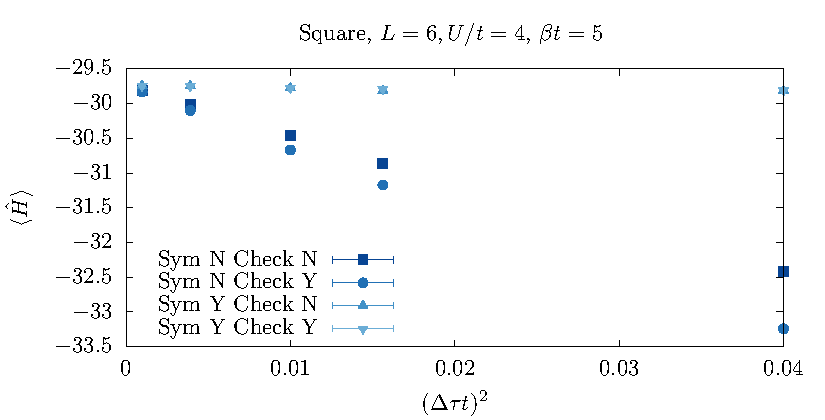
\includegraphics[width=0.49\textwidth]{Figures/Dtau/Dtau.pdf}

        \caption{Analysis of  Trotter systematic error.  Here we consider the $6\times 6$ Hubbard model at $U/t=4$, half-band filling,  inverse temperature $\beta t =5$, and we have used the Hubbard Stratonovich transformation that couples to the z-component of spin.     We provide data for the four combinations of  the logical variables \texttt{Symm}  and \texttt{Checkerboard}.   \texttt{Symm=.true.}    (\texttt{.false.})  corresponds to a symmetric  (asymmetric) choice  of the Trotter decomposition.  \texttt{Checkerboard = .true.}  (\texttt{.false.})   uses (does not use) the  checkerboard   decomposition  for the hopping  matrix. 
  }
        \label{Trotter.fig}
\end{figure}
